%In this chapter, we examine a particular type of molecular systems, namely receptor-ligand systems, consisting of special molecules, so called receptors and ligands.
In this chapter, we examine receptor-ligand-systems, a special type of molecular systems, consisting of so called receptors and ligands. %special/particular
These molecules can interact in such a way that under certain conditions they can bind to each other and afterwards dissociate again.
Such a system is originally Markovian and can be described by a transfer operator.
However, by projecting this operator onto a finite-dimensional state space, the Markov property of the process may be spoiled.

%introduce, present, explain. quantity, occurence
We explain this memory effect, the so called rebinding effect, and examine its influence on the stability of a receptor-ligand-system. We show how this effect can be measured with tools known from chapter \ref{chap:markov}. %its influence on the quantity of binding events of a receptor-ligand-system
In particular, we present a lower bound for the rebinding effect included in a given system as the solution of an optimization problem.
%We are particularly interested in analyzing an optimization problem to find a lower bound for the rebinding effect included in a given kinetics.

%emphasis, focus, is mainly based on, mathematically based. basic/fundamental. knowledge,notations,defs
This chapter highly complies with Weber and Fackeldey\cite{weber2014}.
Additionally, we introduce some fundamental definitions and notations from biochemistry, which are necessary for the understanding of receptor-ligand-systems.
The importance of such systems is illustrated by an outlook of its application in drug design. %becomes clear
%The meaning/importance/relevance of such systems becomes clear by a description/outlook of its application/uses for drug design.
%and involves an approach for nonreversible processes.
%also\cite{weber2012}?

\section{Receptor-Ligand System}
\label{sec:rebinding}

We present a particular molecular system, the \textit{receptor-ligand-system}, and model it mathematically using a differential equation.
We discuss the so called rebinding effect and set in in relation to the recrossing effect known from section \ref{sec:recrossing}.
%a memory effect occuring in this model,
%outlook for later/further investigations
As a motivation, we explain its relevance in the application of drug design.
%As an outlook/motivation.. important application of \textit{drug design} and how the rebinding effect can help to improve the effect/efficiency of drugs. \marginpar{?} NO? just reveals that in reality, we have higher binding affinity, than we thought?stillgood

\subsubsection*{Molecular Dynamics vs Molecular Kinetics}
%\marginpar{Weber p.10}
A molecular system consists of molecules, that are atoms which are connected by \textit{covalent bonds}.
%bla bla.
%The potential energy function, or \textit{energy landscape}, of a molecular system results in a dynamical behaviour on different timescales.
%The fastest timescales (vibrations of covalent bonds) are around $10^{-15}$ seconds. \marginpar{see ..}
%They can  range from 10^-15 seconds for the vibration of covalent bonds, to seconds or even longer (for instance protein folding, ligand binding))
%bla. up to nanoseconds or, for protein folding, up to microseconds or seconds or even longer..
%\\
The motion inside of such a system can be characterized in different ways.
%Such a system can be characterized in different ways. %described/analyzed/characterized
The term \textit{molecular dynamics} denotes the analysis of a \textbf{single} trajectory and is mainly employed in the context of simulations. \marginpar{?}
It means that one initial configuration of the system is fixed and its evolution in time is observed. One example is depicted in figure \ref{fig:conformations}.
It represents \textbf{one} trajectory of a stochastic system. This can give an insight about the structure of the system, like identifying possible metastabilities. However, it is not representative in the sense that a second simulation could yield a completely different trajectory.
In contrast to that, in \textit{molecular kinetics}, an \textbf{ensemble} of trajectories is considered.
Accordingly, it is formulated in terms of densities, concentrations or transition rates.
%These terms cannot be mixed with the trajectory-based approach. Sentences like "trajectory behaves according to transition rate" makes no sense
However, these quantities are related to the molecular dynamics approach as they represent an average of many single realizations of a process.
%These observables/quantities can be understood/interpreted as averages/result of many/infinitely many single rajectories.


\subsubsection*{Receptors and Ligands} \marginpar{references}

In biochemistry, a \textit{receptor} is a molecule, often a protein, that is usually located on the surface of a cell and can receive signals from outside the cell.
A molecule that has the ability to \textit{bind} or \textit{associate} to a receptor is called a \textit{ligand}.
Each receptor will only bind with ligands of a particular structure, which is often referred to as the ``key-lock principle''.
%lock-key
Both receptor and ligand need to have specific complementary geometric shapes that fit exactly into one another, as exemplarily depicted in figure \ref{fig:Protein_ligand_binding}.
%correct size, shape, and charge composition in order to bind and interact with the receptor.

%both of them have specific shape which has to fit to each other
\begin{figure}[!ht]
	\centering
	\includegraphics[width=0.5\textwidth]{figures/receptor_ligand.eps}
	\caption{Ligand (``key'') binds to a receptor (``lock''). Their shapes fit together.}
	\label{fig:Protein_ligand_binding}
\end{figure}

%produce,cause,lead to,provoke,trigger
Such a binding between a receptor and a ligand can \textit{activate} (``unlock'') the receptor by producing some kind of a chemical signal and thereby provoke a physiological response.
For instance, that could be a conformational change in a protein, caused by a hormone binding to it.
%binding energy can lead to conformational change in the receptor, %https://en.wikipedia.org/wiki/Ligand_(biochemistry)
%actual,possible consequences
However, instead of engaging in the actual physiological consequences of a binding, we focus on the \textbf{act} of binding events.
%Thus, we consider a \textbf{ligand binding process}.

%random movements of particles. Brownian motion?
%assume: well-stirred/mixed -> equilibrium. what if starting in non-equilibrium?
%in general, typically
The action of binding is typically reversible\footnote{We remark that in this context, \textit{reversible} means that a ligand can bind and unbind to a receptor, i.e. the reaction can run forward and backward.
%that is bound in a complex has the ability to dissociate from the complex and become unbound again.
In contrary to the mathematical reversible, which means that a process behaves \textbf{equally} when running backwards in time.} through \textit{dissociation} of the involved receptor and ligand.
Ligand binding is a \textit{chemical equilibrium} process, which means that the reaction rates of the binding and dissociating events are equal, once this equilibrium is reached.
From then on, the concentrations of the reactants (ligands) and the products (complexes) are constant.
It is a \textit{dynamic equilibrium}, since reactions take place, even though no net change in the concentrations can be observed.

The binding behaviour of a simple receptor-ligand system is formalized as follows. %\marginpar{kinetics}
A ligand (L) can bind to a receptor (R) and form a receptor-ligand complex (LR) which can dissociate again into its original components. This process can be represented by a reaction equation
%in the following form
\begin{equation}
\label{eq:reaction}
\mathrm{L} + \mathrm{R} \rightleftharpoons \mathrm{LR}.
\end{equation}
%implies,states
Being a process in chemical equilibrium, the law of mass action states that the ratio between the concentration of reactants and products is constant.
The corresponding \textit{dissociation constant} $k_d$ is given by
\begin{equation*}
k_d = \frac{\mathrm{[L]} \cdot \mathrm{[R]}}{\mathrm{[LR]}},
\end{equation*}
%free/unbound
where [L] is the concentration of unbound ligands, [R] is the concentration of unoccupied receptors and [LR]  is the concentration of receptor-ligand complexes.
%where [L], [R] and [LR] represent the concentrations of (L),(R) and (LR), respectively.
%relatively/proportionally
This constant is used to describe the \textit{binding affinity} between a ligand and a receptor, that is how strongly/tightly the ligand can bind to his particular receptor. If the dissociation constant is small, then there are relatively many complexes in comparison to unbound molecules, and for this reason, the binding affinity between the ligand and the receptor is high.
%Affinity is a measure of the tendency of a ligand to bind to its receptor.
The \textit{association constant} $k_a$ is just the inverse of the dissociation constant
\begin{equation*}
k_a = \frac{\mathrm{[LR]}}{\mathrm{[L]} \cdot \mathrm{[R]}}.
\end{equation*}
There are different factors which can influence the binding affinity of a process.
%Firstly, the attraction between receptor and ligand needs to be high. Furthermore, the binding strength needs to be high, that is dissociations should not happen often. ???
%\marginpar{affinity = anziehung + staying in bond + strong rebinding?} NO! only anziehung?
% reasons/values
%The dissociation constant for a particular ligand-protein interaction
It depends on the nature of the constituent molecules, like their shape, size and possible charge.
The binding affinity of a particular ligand-protein interaction can also change significantly with solution conditions (e.g., temperature, pH and salt concentration).
%thus, take a drug at a certain temperature
%These factors can depend on different parameters of the system, like temperature or PH value; but also on the nature of the constituent molecules, like their shape, size and possible charge.
%The rate of binding is called affinity, and this measurement typifies a tendency or strength of the effect.
%https://en.wikipedia.org/wiki/Ligand_(biochemistry)
%For example, a higher temperature leads to a faster movement of the molecules and therefore increases the probability of binding events. \marginpar{but also dissociates faster?}

In general, high-affinity binding results in a higher degree of occupancy for the ligand at its receptor binding site than is the case for low-affinity binding; the residence time (lifetime of the receptor-ligand complex) does not correlate. \marginpar{?}
%https://en.wikipedia.org/wiki/Ligand_(biochemistry)

\subsubsection*{Mathematical Model of Receptor-Ligand-System}

Starting from the reaction equation \eqref{eq:reaction}, we can deduce that the ligand can be found in two different macro states: ``unbound'' (L) or ``bound'' (LR). Then the probabilities of the ligand to be in one of these states can be described by the probability vector $x^T = \frac{1}{s}((\mathrm{[L],[LR]}))$, where $s = \mathrm{[L]} + \mathrm{[LR]} = \textrm{const.}$ is the normalization constant.
This leads to an ordinary differential equation
\begin{equation*}
\dot{x}^T = x^T Q_c.
\end{equation*}
The matrix $Q_c$ consists of the rates of reaction,
\begin{equation*}
Q_c = 
\begin{pmatrix}
-k_a[R] & k_a[R]  \\
k_d      & -k_d
\end{pmatrix},
\end{equation*}
where $k_a$ and $k_d$ are the association and dissociation constants. It corresponds to the transition rate matrix of a Markov chain, that means it describes a \textbf{memoryless} process.
We will later see that this mathematical description of a receptor-ligand-system is not accurate, since in fact, such a process \textbf{will} have some kind of memory.
%does not describe the actual/real long-time behaviour of the system

\begin{figure}[!ht]
	\label{fig:two_states}
	\centering
	\subfigure[Unbound]{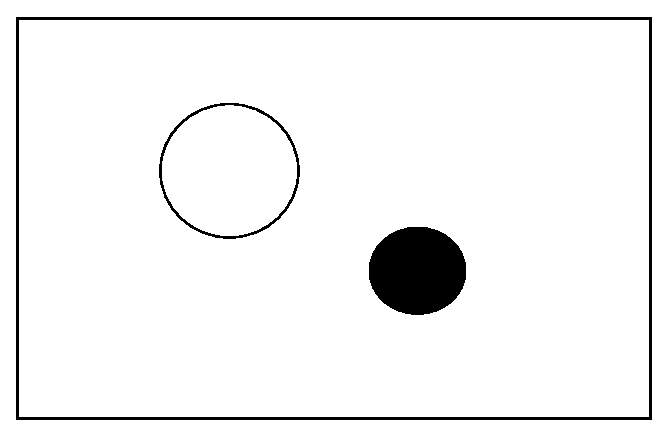
\includegraphics[width=0.25\textwidth]{figures/unbound.eps}}
	\hspace{20pt}
	\subfigure[Bound]{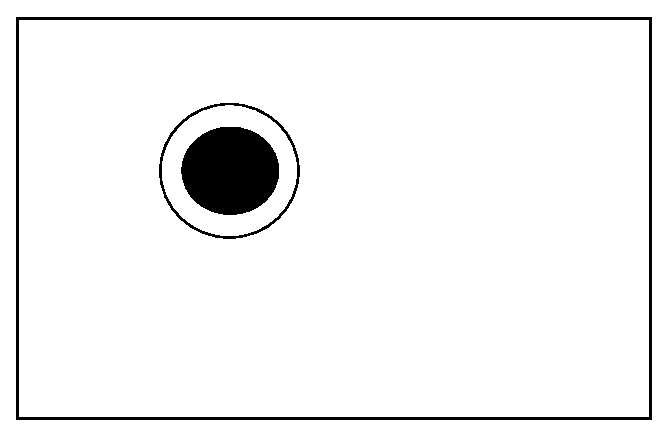
\includegraphics[width=0.25\textwidth]{figures/bound.eps}}
	\caption{Two possible macro states of a ligand-binding system}
	%(unbound, bound)
\end{figure}

The two possible macro states for the easiest case of a ligand-binding-system consisting of one receptor and one ligand are depicted in figure \ref{fig:two_states}. %We discover/detect/notice/remark
We notice that the spatial arrangement of the receptor and the ligand in the unbound case is \textbf{not} included in the above model.
%impact,consequences of that will be seen soon
Therefore, we cannot distinguish if, at a given time, the receptor and the ligand are close to each other or not.

\subsubsection*{Rebinding Effect}

%At the beginning/start, we assume that the molecules are rather good mixed and thus the probability for binding events is rather gleichverteilt.
%But after some time, bindings will occur. And that will lead to memory effects!

%The rebinding effect has been characterized as a \textbf{memory effect} which leads to an additional thermodynamic weight of the bound state.
%Weber quantifying rebinding effect
%occurs when projecting a MD process onto a finite subspace??

%assume: at the beginning well-stirred and thus abstände receptor-ligand gleichverteilt. drugs? :S
%tatsächlich,..
In fact, a stochastic process describing a receptor-ligand system is \textbf{not} necessarily Markovian.
That is due to the spatial arrangement of the system after the dissociating of a receptor-ligand-complex took place.
Shortly after such a dissociating, it is more likely that the corresponding receptor and ligand will bind again, since they are still close to each other.
Such a binding shortly after being dissociated is called a \textbf{rebinding}. The memory effect which thereby occurs is called \textbf{rebinding effect}.
%rebinding event. will vanish, diminish
On large timescales, this effect will vanish since the favorable spatial situation is not necessarily given anymore and the system will be rather mixed again.
%rebinding: rein mathematisch durch die Projektion entstanden?
%oder kann ein Prozess aus anderen Gründen mehr oder weniger Rebinding haben? multivalence
%can or IS spoiled? may be spoiled?
Thus, Markovianity can be spoiled by the rebinding effect.
It is depicted in figure \ref{fig:rebinding}.
\\


\begin{figure}[!ht]
	\label{fig:rebinding}
	\centering
	\subfigure[Spatial constellation shortly after dissociation. The ligand is still \textbf{close} to the receptor.]{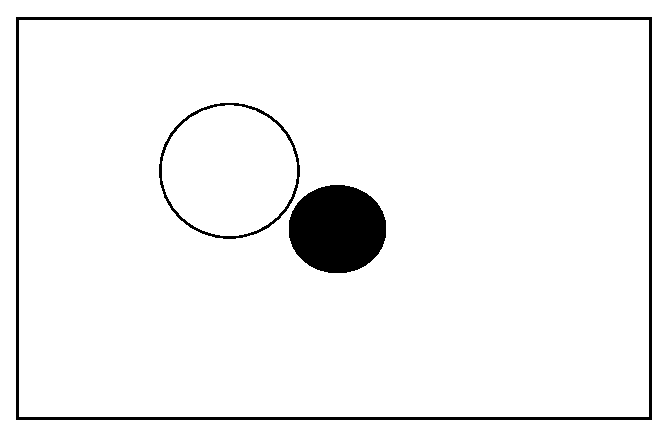
\includegraphics[width=0.25\textwidth]{figures/unbound2.eps}}
	%, increasing the probability of a fast \textbf{rebinding}.
	\hspace{20pt}
	\subfigure[Possible spatial arrangement long time after a dissociation.]{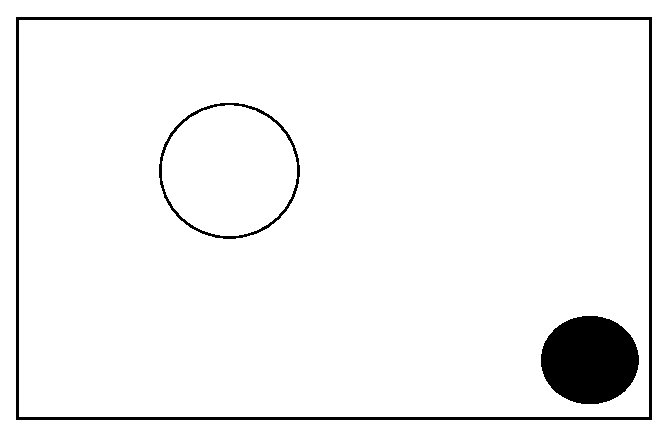
\includegraphics[width=0.25\textwidth]{figures/unbound1.eps}}
	\caption{Rebinding Effect. Two configurations of a system consisting of one receptor and one ligand, represented by the same macro state (``unbound'').}
	%receptor (white) and one ligand (black)
	%(unbound, bound)
\end{figure}

%in molecular systems
The rebinding effect and its occurence in natural science has been described and analyzed by several authors\cite{goldstein1995approximating, vauquelin2010}.
In chemistry, it has been discussed in the context of clustered receptors and clustered ligands\cite{care2011impact}. %\marginpar{multivalence}
%efforts,approaches. quantify the rebinding effect.  mathematical point of view
A mathematical description of the rebinding effect has been realized by Weber et al\cite{weber2012,weber2014}.
%as the rebinding effect occurs by the projection, i.e. by a mathematical concept
%embed it in mathematical context
% and a mathematical point of view.
%from a chemical and a mathematical point of view.

%In chemistry, there are several reasons/factors for the strength/quantity of the rebinding effect discussed (multivalency,..). \marginpar{only math; impact of multivalence}
%(Weber, Chem.)
%recently
The rebinding effect has been discussed to increase the binding affinity of a process.
\marginpar{?}


\subsubsection*{Rebinding Effect vs Recrossing Effect}
The characterization of the rebinding effect reminds us of  the recrossing effect, as described in section \ref{sec:recrossing}.
%We remember the description of the recrossing effect in section \ref{sec:recrossing}.
There, we considered the projection of a possibly continuous process onto a finite state space. This projected process (MSM) was described by a transition matrix, thus being a Markov chain, even though the process actually contained a (short-time) memory. \marginpar{it. error vs reb. eff.}
%There, we had a projected process on macro states described by a transition matrix and thus being a Markov chain. But in reality, the (clustered) process was not memoryless.
The same phenomena occurs with the rebinding effect.
We have a process which is \textbf{modelled} by a Markov chain, even though the process actually \textbf{has} a memory.
%We have a transition matrix, even though our process has a memory.
We can interpret the two states of the ligand-binding-system as macro states resulting from the projection of a process on a larger state space (for instance, including more informations about the spatial situation of the receptor and the ligand).
%(for instance, containing informations about the spatial coordinates of the (contributing) molecules).
In this case, the rebinding effect originates from the loss of information caused by the projection and therefore, qualitatively corresponds to the recrossing effect. %\marginpar{quant. same?}
\\

Thus, the rebinding effect coincides with the recrossing effect in the special context of a receptor-ligand-system. %for the special
%or the same? justified,caused,stem. respectively
The different nomenclatures are justified by the use in their original context. While the term recrossing effect denotes the act of \textbf{recrossing} an energy barrier, the term rebinding effect denotes the \textbf{rebinding} of two molecules in a receptor-ligand-system. Such a system can also be represented by a potential energy function, having energy minima around the bound (closest possible distance) and unbound state (farthest possible distance).
\\

%spatial situation/arrangement
In chapter \ref{chap:meta}, we learned that a fuzzy clustering should be chosen instead of a hard one, in order to yield a valid projection.
%Accordingly
Therefore, we are going to include the spatial situation of the system by introducing degrees of membership, which can be interpreted as ``intermediate'' states such as ``almost bound''.
%certain, high. For this aim
%In this case, could correspond
In this sense, an unbound state with a high degree of membership to the bound state can be interpreted as a a ligand being \textbf{close} to a receptor, for instance shortly after dissociating.
\\

In the next sections, we are going to quantify this effect by embedding the molecular system and its projection into the mathematical framework established in the first two chapters.
%known,established

\subsubsection*{Application: Drug Design} %\marginpar{structure-based vs. rational DD}

%inventive process of finding new medications
%describes,connotes,denotes. Most commonly
The term \textit{drug design} denotes the development of new medications based on the knowledge of a biological target, playing the role of the receptor.
Drug design is basically about designing a molecule which is
%complementary to the binding site of target
complementary in shape and charge to the biomolecular target and therefore will bind to it, see Str{\o}mgaard et al\cite{stromgaard2002}.
More precisely, drug design describes the design of ligands, that is molecules that will bind tightly to the given target, see Tollenaere\cite{tollenaere1996}.
In general, we can distinguish between the following two most common functionalities of drugs.
%kind/types of drugs.
\begin{itemize}
%agonists. full agonists vs partial agonists w/ different efficacy b/w 0 and 100
\item \textbf{\textsf{Activators}} are able to activate, or even deactivate, a receptor and result in a strong biological response.
An example for such a drug is morphine, which acts directly to the central nervous system, mimics the actions of endorphins and thereby reduces pain.
\item \textbf{\textsf{Inhibitors}} bind to a receptor without activating it. Though, as they ``block'' the binding sites of receptors, they prevent possibly disease causing particles to bind.
A well-known example are protease inhibitors, a class of antiviral drugs that are widely used to treat HIV and hepatitis C.
%disease causing ... objects ../particles/molecules/enzymes
\end{itemize}

%aimed,wished,required,needed
Independently of the fact whether a drug activates or inhibits receptors, a high binding affinity is required in order to be an efficient drug.
The central dogma of receptor pharmacology (``occupation theory'') is that a drug effect is directly proportional to the number of receptors that are occupied. Furthermore, a drug effect ceases as a drug-receptor complex dissociates.
Thus, a low binding affinity needs to be compensated by a higher concentration of ligands.
%of Wirkstoff
Though, high concentrations should be avoided, because of possible side effects.
%and other reasons
%If the binding affinity of a drug is too low, a higher concentration of it is needed,
%in order to be effective, higher dose
%which is undesired because of possible side effects.
Accordingly, the most fundamental goal in drug design is to predict whether a given molecule will bind to a target and if so how strongly.

%The drug is often a small molecule which can bind to a protein molecule (target/disease/receptor) and thus activates or inhibits its function (disease modifying).
%is about developing
%target = receptor; drug = ligand.. simplified model
%disease: have a bad molecule/protein/receptor which can bind to a human cell and create sickness.
%tendency to bind

%high binding affinity, measure of the strength of the chemical bond.
%It means that the designed ligands should easily bind to the receptors, remain in a binding or rebind quickly after dissolving.
%There are many factors that influence/affect the binding affinity of a drug/ligand, such as ... .
%The rebinding effect has been recently investigated to increase the binding affinity of a ligand, mathematically described by Weber et al\cite{weber2012, weber2014} as well as chemically by e.g. Vauqelin\cite{vauquelin2010}. This effect will be examined in this thesis. As a \textit{high} rebinding effect is aimed/wished, we will derive a lower bound for this effect, i.e. we will \textit{minimize} it.
%several factors for high binding affinity: like good shape, multivalency

%A drug consists of ligands which should bind to the receptors of the virus. If the drug creates many bindings, %the virus is "bound" and cannot attack the human (cell?) anymore. Thus, many bindings are favorable

%\subsubsection*{Occupation Theory} https://en.wikipedia.org/wiki/Receptor_(biochemistry)
%Affinity is a measure of the tendency of a ligand to bind to its receptor. Efficacy is the measure of the bound ligand to activate its receptor.
%Affinity: The ability of a drug to combine with a receptor to create a drug-receptor complex.
%Efficacy: The ability of a drug-receptor complex to initiate a response.

%\subsubsection*{Multivalence} \marginpar{covalent bonds?}
%Multivalent receptors possible or of interest?

%Multivalent ligands consists of several molecules connected by (inert?) so called ``linkers''.
%Bivalent ligands consists of two molecules connected by an (inert?) linker.

%In general, multivalent ligands have a higher binding affinity because of the favorable spatial arrangement.
%If one of the ligands dissolves, then the other (connected) ligands still hold it in place (close to receptor).

%According to that
%Furthermore, systems consisting of multivalent receptors and multivalent ligands are discussed to have a high rebinding effect.
%\pagebreak